%===============================================================================================
%		Technische Archiktur
%===============================================================================================

\chapter{Technische Architektur}
\label{sec:TechnicalArchitectureChap}

%-----------------------------------------------------------------------------------------------
%		Technische Infrastruktur
%-----------------------------------------------------------------------------------------------

\section{Technische Infrastruktur}
\label{sec:TechnicalInfrastructure}

Die technische Infrastruktur beschreibt die Umgebung, die f�r das Arbeiten mit \LibName{} ben�tigt wird, wie in der folgenden Abbildung gezeigt:

\begin{figure}[H]
	\centering
		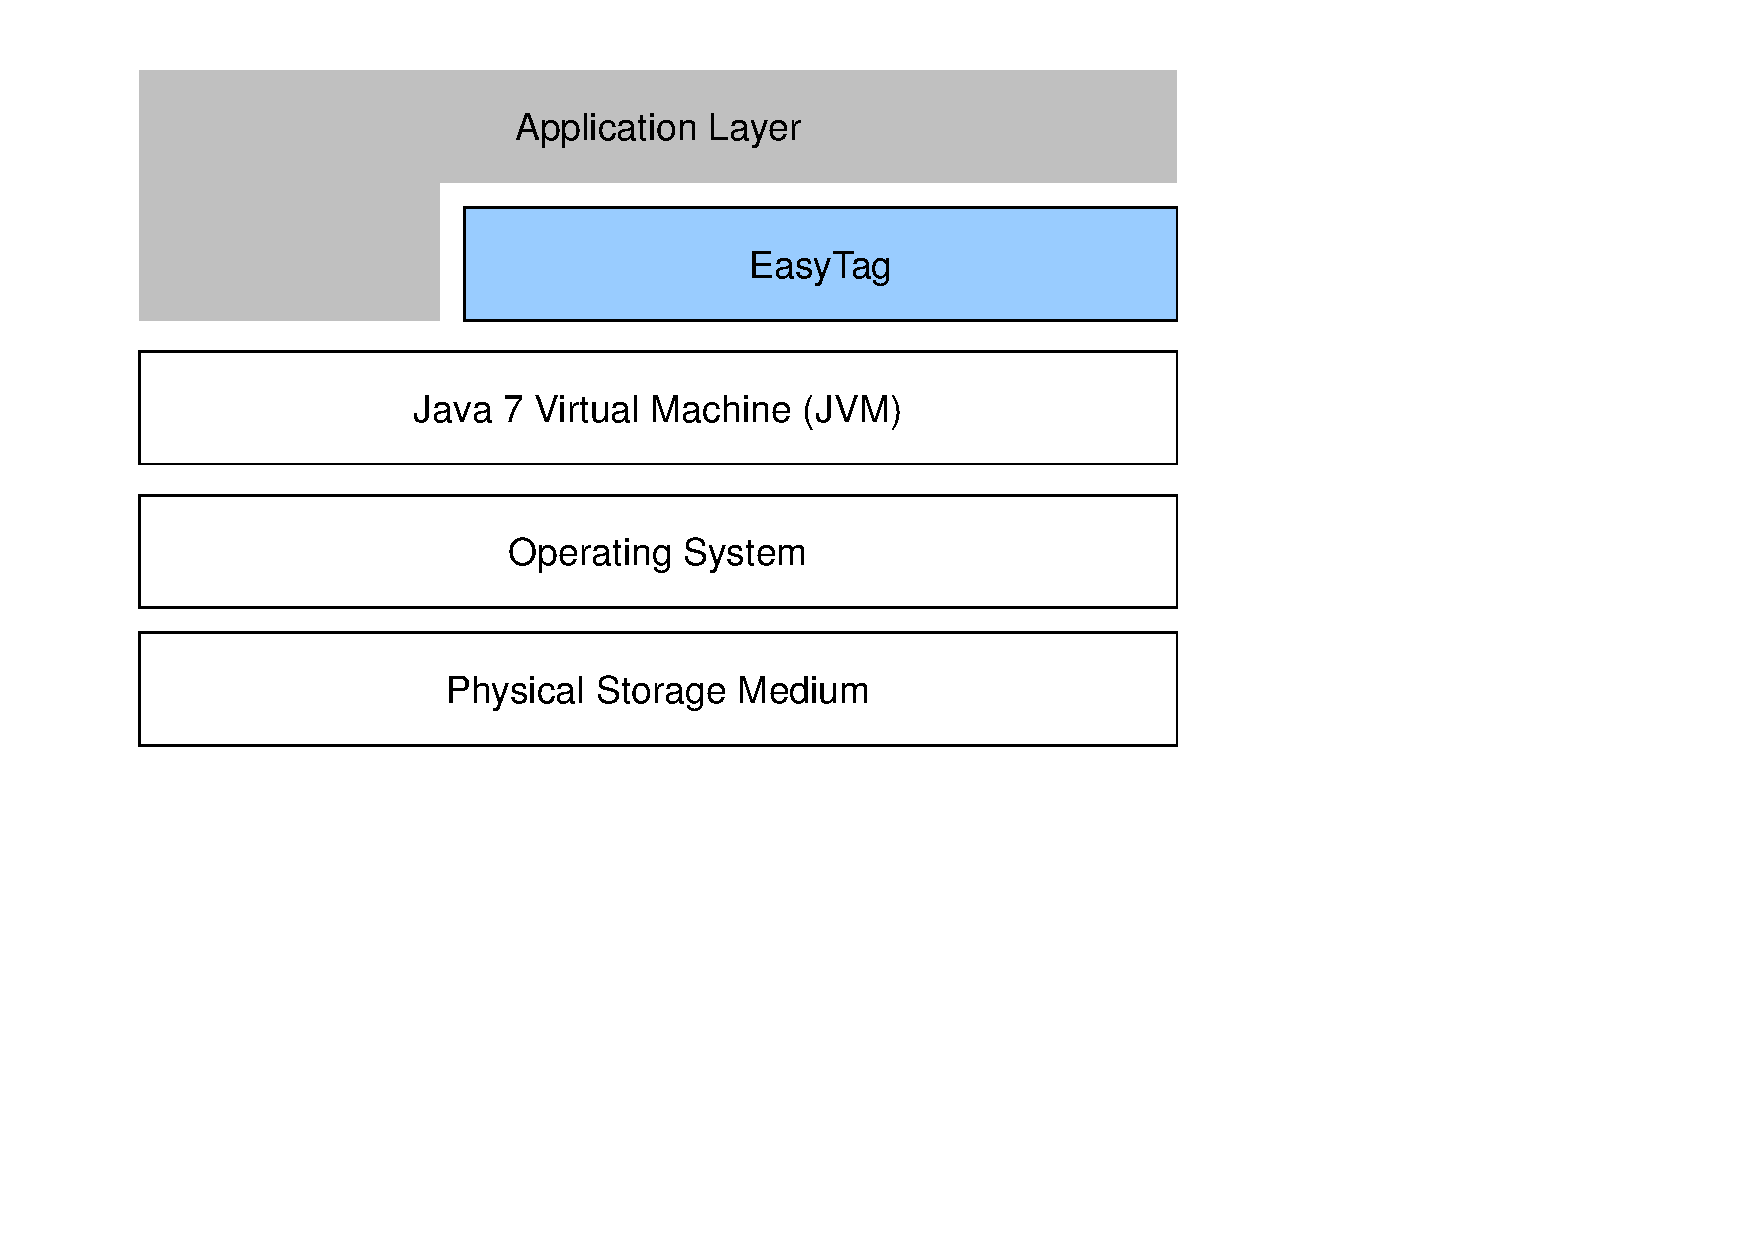
\includegraphics[width=1.00\textwidth]{Figures/Part_II/II_1_TechnicalInfrastructure.pdf}
		\caption{Technische Infrastruktur von \LibName{}}
	\label{fig:5_3_SCH_TechnicalInfrastructure}
\end{figure}

Die technische Schichtenstruktur kann als Abh�ngigkeits- und Kommunikationsstruktur interpretiert werden. Der Applikations-Layer basiert auf \LibName{} w�hrend sowohl \LibName{} als auch der Applikations-Layer die \JavaVersion{} benutzen. \JavaVersion{} greift auf das Betriebssystem zu, welches Dienste zum Zugriff auf das physische Medium bietet.

Die Schichten sollten dabei nur auf benachbarte Schichten zugreifen.

%-----------------------------------------------------------------------------------------------

\subsection{Application Layer}
\label{sec:ApplicationLayer}

Der Application Layer ist die Software, die \LibName{} zum Extrahieren und Schreiben von Metadaten nutzt. Es handelt sich um eine Java-Anwendung, mindestens f�r \JavaVersion{} entwickelt worden ist. Sie nutzt nat�rlich dar�ber hinaus andere Java-Funktionalit�t und Libraries. Es kann sich um eine Java-SE-Desktop-Applikation oder auch eine Java-EE-Server-Applikation handeln.

%-----------------------------------------------------------------------------------------------

\subsection{\LibName{}}
\label{sec:LibName}

In der Abbildung bezeichnet \LibName{} alle Laufzeitkomponenten der Library \LibName{}. Diese Komponenten werden vom Application Layer aufgerufen und genutzt. \LibName{} selbst ist eine reine Java Library, die auf der \JavaVersion{} Java Virtual Machine (JVM) l�uft. Sie kann somit nicht mit �lteren Java-Versionen eingesetzt werden.

%-----------------------------------------------------------------------------------------------

\subsection{Java Virtual Machine (JVM)}
\label{sec:JavaVirtualMachineJVM}

\LibName{} ben�tigt eine Java Virtual Machine (JVM). \LibName{} wird in \JavaVersion{} entwickelt und ist daher nicht auf fr�heren Versionen nutzbar.

%-----------------------------------------------------------------------------------------------

\subsection{Betriebssystem}
\label{sec:OperatingSystem}

Die JVM l�uft auf jedem Betriebssystem, das \JavaVersion{} unterst�tzt. Daher entkoppelt die JVM \LibName{} vom Betriebssystem. Es gibt jedoch einige Systemfunktionalit�ten wie Prozess- und Threadmanagement ebenso wie Dateisystemzugriff, die teilweise vom Betriebssystem abh�ngen.

%-----------------------------------------------------------------------------------------------

\subsection{Physisches Speichermedium}
\label{sec:PhysicalStorageMedium}

\LibName{} greift auf Daten zu, die auf einem physischen Speichermedium gespeichert sind. Seine Lage oder Art ist unterschiedlich. In vielen F�llen handelt es sich um eine Datei auf einer Festplatte, es k�nnte sich aber auch um eine entfernt gespeicherte Ressource, Hauptspeicher oder eine Datenbanktabelle in einer entfernten Datenbank handeln.

Der Application Layer muss bei Verwendung von \LibName{} niemals selbst auf das physische Medium zugreifen. \LibName seinerseits nutzt die \JavaVersion{}, diese das Betriebssystem, um auf die Daten des Mediums zuzugreifen.

%-----------------------------------------------------------------------------------------------
%		Technische Basiskomponenten
%-----------------------------------------------------------------------------------------------

\section{Technische Basiskomponenten}
\label{sec:TechnicalBasis}

Technische Basiskomponenten dienen nur als Hilfsmittel oder Rahmen der Umsetzung der fachlichen Inhalte von \LibName{}. Unter ``fachliche'' Inhalte wird das Lesen und Schreiben von Metadaten und das Lesen von Container-Daten verstanden. Die daf�r notwendigen technischen Basiskomponenten werden hier kurz aufgef�hrt:
\begin{itemize}
	\item Logging
	\item Service-Locator
	\item Utility
	\item Verwaltung von Erweiterungen
\end{itemize}

Details zu diesen Komponenten findet sich in \SectionLink{sec:Design}.

%###############################################################################################
%###############################################################################################
%
%		File end
%
%###############################################################################################
%###############################################################################################